\section{From face correlation to an odd row coefficient}
\label{sec:inner-box}

Proposition~\ref{prop:correlation} gives a low-degree field $L$ with
$\E\mathfrak d_X(L)\ge1/(4T)$. We will show that this correlation
forces a large odd Fourier coefficient in one row of the original field
$h$, as required by Theorem~\ref{thm:inner}. We first choose $m$ large enough to partition
the Fourier--Hermite terms of $L_x$: each nonzero term either has positive degree
in $c_x$, or carries equal odd frequencies in two rows
$B^i_{x_{-i}}$ and $B^j_{x_{-j}}$. Equal frequencies turn the two row
factors into a character of their sum. Restriction to a random smaller box
will then separate the other variables, allowing the two kinds of terms
to be estimated by centering and by a four-corner Fourier identity.

Throughout this Section, $\sigma,\delta,\eta,R,s,T$ are the constants of
Proposition~\ref{prop:correlation}, already chosen independently of
$m,n$ and of the affine alphabet. All expectations include the weighted
proof index $\xi$, unless explicitly conditioned on it. We use only
averaged test bounds; individual indices need not satisfy those bounds.

Let
\[
 \mathcal R=\{(i,y):i\in[m],\ y\in[n]^{[m]\setminus\{i\}}\},
 \qquad M=|\mathcal R|=mn^{m-1}
\]
be the set of rows. For a family of frequencies
$\boldsymbol\alpha=(\alpha_r:r\in\mathcal R)$, write
$\chi_{\boldsymbol\alpha}(B)=\prod_r\chi_{\alpha_r}(B_r)$ and
$S_i=\{y:\alpha^i_y\ne0\}$. Thus $S=(S_i)_i$ is the exact row mask,
and $|S|=\sum_i|S_i|$ is the row degree. At a fixed proof index, the
Fourier--Hermite expansion of the projected field is
\begin{equation}\label{eq:box-expansion}
 L_x(B,c)=
 \sum_{\substack{|I|\le s\\|S(\boldsymbol\alpha)|\le Rm}}
 \widehat h_x(\boldsymbol\alpha,I)
 \chi_{\boldsymbol\alpha}(B)\psi_I(c).
\end{equation}
This is a finite sum. Coefficients and the row frequency spaces may depend
on $\xi$; the sets of row positions and Hermite indices do not. We select
components using only $x,I,S$. Counting row masks and Hermite indices,
without counting the possible values of the nonzero frequencies,
will keep the coefficient estimates independent of the alphabet.

\subsection{Gauge identities and a partition selected by masks}

We use two symmetries of $h$ to find these equal, odd local frequencies.
First fix distinct axes $i,j$ and a tuple
$q\in[n]^{[m]\setminus\{i,j\}}$. For $a\in D(A)$, add $a$ to every row
$B^i_y$ with $y_{-j}=q$ and every row $B^j_y$ with $y_{-i}=q$.
Call the resulting array $B^{(a)}$. At a point $u\in X$, either both
additions occur or neither occurs, so $B^{(a)}(u)=B(u)$. Consequently
$h_x(B^{(a)},c)=h_x(B,c)$. Orthogonality, or a change of variables in the
Fourier coefficient, shows that every nonzero coefficient satisfies
\begin{equation}\label{eq:cylinder-gauge}
 \sum_{y:y_{-j}=q}\alpha^i_y
 +\sum_{y:y_{-i}=q}\alpha^j_y=0
 \qquad\text{in }D(A)^*.
\end{equation}
Indeed, otherwise some $a$ makes the character change sign while the
function remains unchanged.

For the second symmetry fix a row $r=(i,v)$ and put
$k_u=\one_{\{u_{-i}=v\}}$. This is a codeword in $\C$. Let $B+1_r$
denote addition of the constant-one affine function in this row, and let
$D_kc=((-1)^{k_u}c_u)_{u\in X}$. Translation of a codeword argument by
$k$ gives the exact identity
\[
 P_{c+\sigma g,\eta\lambda}(z+k)
 =P_{D_kc+\sigma D_kg,\eta\lambda'}(z),
 \qquad \lambda'_z=\lambda_{z+k}.
\]
The Gaussian vectors $D_kg$ and $\lambda'$ have the original joint law.
The proof is a function of the resulting Boolean table on $A$, so
\[
 F_{B+1_r}(c)=F_B(D_kc),\qquad
 h_x(B+1_r,c)=(-1)^{k_x}h_x(B,D_kc).
\]
The derivative in the second equality supplies its displayed sign.
Since $\psi_I(D_kc)=(-1)^{\sum_u k_u I_u}\psi_I(c)$, every nonzero
coefficient also satisfies
\begin{equation}\label{eq:row-gauge}
 \alpha_r(1)\equiv k_x+\sum_{u\in X}k_uI_u\pmod2.
\end{equation}
These identities hold separately for every proof index and for every
alphabet.

Choose $m>s+1$ so large that
\begin{equation}\label{eq:choose-m}
 \binom{m-s}{2}>Rm.
\end{equation}
Partition the terms of $L_x$ as follows. Those with $I_x>0$ form class
$0$. For each remaining pair $(I,S)$, choose two axes $i<j$ subject to:
\begin{enumerate}[label=(\roman*),leftmargin=*]
 \item No $u$ with $I_u>0$ satisfies $u_{-i}=x_{-i}$ or
       $u_{-j}=x_{-j}$.
 \item Among rows of $S_i$ above $x_{-ij}$, the only permitted row is
       $x_{-i}$; among rows of $S_j$ above $x_{-ij}$, the only permitted
       row is $x_{-j}$.
\end{enumerate}
Such a pair exists. Since $I_x=0$, each positive Hermite support point
differs from $x$. It can agree with $x$ after deleting an axis for at
most one axis, so at most $s$ axes are forbidden by (i). A nonlocal row
$y\in S_i$, $y\ne x_{-i}$, obstructs (ii) for at most one other axis
$j$: its coordinates must differ from $x_{-i}$ only at $j$. Thus all
masks together forbid at most $Rm$ unordered pairs. Inequality
\eqref{eq:choose-m} leaves an admissible pair.

Fix an ordering of the pairs and choose the first admissible one. This
rule uses only $x,I,S$, never the values of the nonzero frequencies.
Assign the entire exact-mask/Hermite component to that pair class.
For a nonzero term in class $(i,j)$, apply~\eqref{eq:cylinder-gauge}
with $q=x_{-ij}$. Condition (ii) leaves only the two local frequencies,
so they are equal. Apply~\eqref{eq:row-gauge} to
$r=(i,x_{-i})$. Here $k_x=1$ and condition (i) makes the Hermite sum
zero. Therefore
\begin{equation}\label{eq:matching-odd}
 \alpha^i_{x_{-i}}=\alpha^j_{x_{-j}},
 \qquad \alpha^i_{x_{-i}}(1)=1.
\end{equation}
In particular both local rows really occur in the mask. Equality and
oddness are consequences of the two symmetries, rather than extra
conditions used to filter individual frequencies.

Write $L^a$ for the class arrays, with
$a\in\mathcal K=\{0\}\cup\{(i,j):1\le i<j\le m\}$, and set
\begin{equation}\label{eq:class-target}
 d_0=\frac{1}{4T(1+\binom m2)}.
\end{equation}
By subadditivity of $\mathfrak d_X$ and Proposition~\ref{prop:correlation},
\begin{equation}\label{eq:class-correlation-lower}
 \frac1{4T}\le\E\mathfrak d_X(L)
 \le\sum_{a\in\mathcal K}\E\mathfrak d_X(L^a).
\end{equation}
It will suffice to show, under failure of the asserted row-atom
conclusion, that every summand is strictly less than $d_0$.

\subsection{Localization to a random subbox}

Let $2\le\ell<n$, with both integers to be chosen later. Independently
on each axis choose a uniform $\ell$-element subset $Y_i\subset[n]$,
and put $Y=\prod_iY_i$. The average of a uniform point in $Y$, over
this random choice, is uniform in $X$. For every deterministic array
$v$,
\begin{equation}\label{eq:box-restriction}
 \mathfrak d_X(v)\le\E_Y\mathfrak d_Y(v|_Y).
\end{equation}
To prove this, choose face signs attaining $\mathfrak d_X(v)$, restrict
them to $Y$, and use that the original correlation is the average of
their restricted correlations. The absolute value of the average is at
most the average of the absolute values. This is a pointwise assertion
and allows the maximizing face signs to depend on the full array.

For $x\in Y$, retain from $L^a_x$ only those terms whose positive
Hermite support on $Y$ is contained in $\{x\}$ and whose masked rows
on the faces of $Y$ are contained in
$\{(r,x_{-r}):r\in[m]\}$. Denote the retained field by $v^a_x$.
Equivalently, $v^a_x=Q^{a,Y}_xh_x$, where $Q^{a,Y}_x$ is an
orthogonal projection selecting complete exact-mask/Hermite components.
In particular its choice depends only on $a,Y,x,I,S$.

Conditional on a uniform point of $Y$ being $x$, the subsets $Y_i$ are
independent uniform $\ell$-subsets containing $x_i$. For a fixed
point $u\ne x$, membership in $Y$ requires that at least one particular
value other than $x_i$ be selected, so its conditional probability is
at most $(\ell-1)/(n-1)$. The same assertion holds for a face tuple
different from the corresponding face of $x$. A term has at most $s$
positive Hermite support positions and $Rm$ masked rows. A union bound,
followed by orthogonality for fixed $x,Y$, therefore gives
\begin{align}
 \E\E_{x\in Y}|L^a_x-v^a_x|^2
 &\le \sigma^{-2}(s+Rm)\frac{\ell}{n-1},
 \label{eq:localization-l2}\\
 \E\E_{x\in Y}|v^a_x|^2&\le\sigma^{-2}.
 \label{eq:retained-energy}
\end{align}
For the first inequality one can sum the squared coefficients of
$L^a_x$ multiplied by their conditional removal probabilities; their
total, averaged over uniform $x$ and $\xi$, is at most $\sigma^{-2}$.
For the second, each retained projection contracts the squared norm
of $h_x$, and then one averages over $x,Y,\xi$. Thus the expected
normalized $L^1$ loss in localization is at most
\begin{equation}\label{eq:localization-loss}
 e_{\mathrm{loc}}=
 \sigma^{-1}\sqrt{(s+Rm)\frac{\ell}{n-1}}.
\end{equation}
No pointwise bound on a retained field is needed here.

There are two useful conditional descriptions. For class $0$, condition
on $\xi,Y$, all rows $B$, and all Gaussians outside $Y$. Each $v^0_x$
is then a function of $c_x$ alone, and its conditional mean is zero:
every retained Hermite term has $I_x>0$ and no other positive index
on $Y$.

For class $(i,j)$, condition on $\xi,Y$, all Gaussians, all tables
other than $B^i,B^j$, and the rows of those two tables outside the faces
of $Y$. Call this background $\mathcal F_{ij,Y}$. The remaining rows
of these two tables are still independent and uniform. Localization
and~\eqref{eq:matching-odd} give, for each $x\in Y$, a function
$V_x:D(A)\to\R$, determined by this background, such that
\begin{equation}\label{eq:local-sum-slice}
 v^{ij}_x=V_x(B^i_{x_{-i}}+B^j_{x_{-j}}),
 \qquad
 V_x(b)=\sum_{\alpha:\alpha(1)=1}\widehat V_x(\alpha)\chi_\alpha(b).
\end{equation}
Indeed, a retained term has no other on-subbox row in either table,
and its two local character factors multiply to the character of their
sum. Thus $V_x$ is independent of the sampled values of every
on-subbox row in tables $i,j$. The slice norm
$\|V_x\|_2$ and its maximum Fourier coefficient are functions of
$\mathcal F_{ij,Y}$ as well. Integrating the two local rows makes
their sum uniform, and hence~\eqref{eq:retained-energy} says
\begin{equation}\label{eq:slice-energy}
 \E\E_{x\in Y}\|V_x\|_2^2\le\sigma^{-2}.
\end{equation}

\subsection{A coefficient estimate with no dependence on the alphabet}

The next estimate connects the projected slices to the original field.
For an axis $i$ and point $x$, put $r=(i,x_{-i})$ and define the
original maximum odd row coefficient by
\[
 a_{x,i}(B_{\ne r},c)=
 \max_{\alpha:\alpha(1)=1}
 \left|\E_{b\in D(A)}h_x(B[r\leftarrow b],c)\chi_\alpha(b)\right|.
\]
This is a function only of the indicated background and the proof
index. Its pointwise upper bound is $\sqrt N/\sigma$.

\begin{lemma}[Uniform transfer through the selected projection]
\label{lem:projected-row-atom}
Let $Q_x^Y$ select any collection of complete exact-mask/Hermite
components with $|I|\le s$, using only $x,Y,I,S$.
For a fixed axis $i$ let $q_{x,i}^Y$ be the maximum odd row coefficient
of $Q_x^Yh_x$ in $r=(i,x_{-i})$, with the other rows and $c$ held fixed.
Then
\begin{equation}\label{eq:projector-maximum}
 \E\E_{x\in Y}q_{x,i}^Y
 \le C_0\left(\E\E_{x\in X}a_{x,i}^2\right)^{1/2},
 \qquad C_0=4^M\binom{N+s}{s}.
\end{equation}
The estimate is valid for every weighted distribution of proof indices.
\end{lemma}
\begin{proof}
For a row $t$, write $E_t$ for averaging that row uniformly. The
projection onto an exact mask $S\subseteq\mathcal R$ is
\[
 P_S=\prod_{t\in S}(\operatorname{Id}-E_t)
       \prod_{t\notin S}E_t.
\]
The projection onto the Hermite index $I$ is
\[
 H_Iu(B,c)=\psi_I(c)\E_{c'}\psi_I(c')u(B,c').
\]
There are $2^M$ masks and $\binom{N+s}{s}$ multi-indices with
$|I|\le s$. Thus $Q_x^Y$ is a sum of at most their product of
operators $P_SH_I$.

Taking a Fourier coefficient in the distinguished row $r$ commutes with
all the other row averages. If $r\notin S$, the average $E_r$
annihilates every odd coefficient. If $r\in S$, the factor
$\operatorname{Id}-E_r$ leaves such a coefficient unchanged. Expand
the remaining factors $\operatorname{Id}-E_t$ into signed averages;
there are at most $2^M$ terms. Each term averages some of the other
rows without changing the distinguished frequency. For one such term,
its maximum odd coefficient is consequently bounded by
\[
 |\psi_I(c)|\,
 \E_{c',\,\text{averaged rows}}
       |\psi_I(c')|\,a_{x,i}(B'_{\ne r},c').
\]
This follows by moving the maximum inside the absolute-value integral;
no sum over row frequencies is introduced. At fixed $\xi,x$, average
the output $c$ and all the other output rows. Uniform row averages
preserve the product measure, $\E|\psi_I(c)|\le1$, and
Cauchy--Schwarz gives
\[
 \E_{B_{\ne r},c'}|\psi_I(c')|a_{x,i}(B_{\ne r},c')
 \le\left(\E_{B_{\ne r},c'}a_{x,i}^2\right)^{1/2}.
\]
The bound is independent of $I,S,Y$. Summing at most
$4^M\binom{N+s}{s}$ expanded terms proves the corresponding bound at
fixed $\xi,x,Y$. Finally apply Cauchy--Schwarz to the probability
measure on $\xi,Y,x\in Y$, and use the uniform marginal of $x$.
This proves~\eqref{eq:projector-maximum}, including arbitrary weights
on $\xi$. Only counts of positions, masks and Hermite indices entered
the constant.
\end{proof}

Suppose, for a contradiction, that the row-atom conclusion in
Theorem~\ref{thm:inner} fails for positive constants $p,\theta$ to be
chosen at the end. In this notation the failed assertion is
\[
 \Prob_{\xi,x,i,B_{\ne(i,x_{-i})},c}[a_{x,i}\ge\theta]<p.
\]
Since $i$ is uniform, for each fixed axis $i$ this event has probability
less than $mp$. The pointwise bound on $a_{x,i}$ gives
\begin{equation}\label{eq:original-atom-square}
 \E\E_{x\in X}a_{x,i}^2\le D,
 \qquad D=\theta^2+\frac{mpN}{\sigma^2}.
\end{equation}
This is only an averaged estimate in $x,\xi$, which is exactly the
estimate required in Lemma~\ref{lem:projected-row-atom}.

For a retained pair class use $Q_x^Y=Q_x^{ij,Y}$ and the distinguished
axis $i$. From~\eqref{eq:local-sum-slice}, its coefficient in the
row $B^i_{x_{-i}}$, when the other local row has value $b'$, is
$\widehat V_x(\alpha)\chi_\alpha(b')$. The maximum magnitude is
therefore precisely
$q_x=\max_{\alpha:\alpha(1)=1}|\widehat V_x(\alpha)|$, independently
of $b'$ or any other remaining row. Equations
\eqref{eq:projector-maximum}--\eqref{eq:original-atom-square} imply
\begin{equation}\label{eq:slice-atom-probability}
 \E\E_{x\in Y}q_x\le C_0\sqrt D,
 \qquad
 \Prob[q_x>\gamma]\le\frac{C_0\sqrt D}{\gamma}
\end{equation}
for every $\gamma>0$. The probability here is over a uniform point
of $Y$ and its slice background.

\subsection{Bounded arrays and background-measurable slice operations}

For $A_0>0$, let $\operatorname{clip}_{A_0}(z)=
\max(-A_0,\min(z,A_0))$. We use
\begin{equation}\label{eq:clip-elementary}
 |z-\operatorname{clip}_{A_0}(z)|\le z^2/A_0.
\end{equation}

For class $0$, use its conditional description above and set
\[
 w^0_x=\operatorname{clip}_{A_0}(v^0_x)
       -\E_{c_x}\operatorname{clip}_{A_0}(v^0_x).
\]
Here the conditional expectation fixes all rows and the Gaussians
outside $Y$. Since $\E_{c_x}v^0_x=0$, inequality
\eqref{eq:clip-elementary} bounds both the clipping loss and the
absolute value of the subtracted mean. Thus
\begin{equation}\label{eq:class-zero-processing}
 |w^0_x|\le2A_0,\qquad
 \E\E_{x\in Y}|v^0_x-w^0_x|\le\frac{2\sigma^{-2}}{A_0}.
\end{equation}
Conditioned on that common background, the variables $w^0_x$, $x\in Y$,
depend on distinct independent Gaussians and have mean zero.

For class $(i,j)$, operate on the entire slice $V_x$ as follows:
\begin{enumerate}[label=(\roman*),leftmargin=*]
 \item Set the slice to zero if $\|V_x\|_2>H$.
 \item Set it to zero if $q_x>\gamma$.
 \item Clip every value of a remaining slice to $[-A_0,A_0]$.
\end{enumerate}
Both discard decisions depend only on $\mathcal F_{ij,Y}$. In
particular, a decision is made from the function of the free sum
variable and is independent of the sampled local rows. Let $W_x$ be
the resulting slice and
$w^{ij}_x=W_x(B^i_{x_{-i}}+B^j_{x_{-j}})$.

Write $\nu_x=\|V_x\|_2$. The first discard costs at most
\[
 \E\E_{x\in Y}\nu_x\one_{\{\nu_x>H\}}
 \le H^{-1}\E\E_{x\in Y}\nu_x^2\le\frac{\sigma^{-2}}H.
\]
For the second discard, Cauchy--Schwarz,
\eqref{eq:slice-energy} and~\eqref{eq:slice-atom-probability} give
the bound
\begin{equation}\label{eq:atom-discard-loss}
 e_{\mathrm{atom}}=
 \sigma^{-1}\sqrt{C_0/\gamma}\,D^{1/4}.
\end{equation}
Indeed its loss is at most
$\E\E_{x\in Y}\nu_x\one_{\{q_x>\gamma\}}$, regardless of whether
the first discard has already occurred. The last clipping operation
costs at most $\sigma^{-2}/A_0$ by~\eqref{eq:clip-elementary}.
Consequently
\begin{equation}\label{eq:pair-processing-loss}
 \E\E_{x\in Y}|v^{ij}_x-w^{ij}_x|
 \le\frac{\sigma^{-2}}H+e_{\mathrm{atom}}+
       \frac{\sigma^{-2}}{A_0}.
\end{equation}

Every processed slice has absolute bound $A_0$ and $L^2$ norm at most
$H$. For a slice surviving both discards, its clipping error in
conditional $L^1(D(A))$ is at most $H^2/A_0$. Each Fourier coefficient
changes by at most this amount. Before clipping the spectrum was odd
and all its coefficients had magnitude at most $\gamma$, so, for all
frequencies,
\begin{equation}\label{eq:processed-slice-bounds}
 \|W_x\|_2\le H,\qquad
 \max_\alpha|\widehat W_x(\alpha)|\le\eps_0,
 \qquad \eps_0=\gamma+H^2/A_0.
\end{equation}
Discarded slices satisfy the same bounds. Symmetric clipping in fact
preserves oddness, since $V_x(b+1)=-V_x(b)$, although the following
estimate only needs the bound for all coefficients.

\subsection{Box Cauchy--Schwarz and the independent squares}

We prove the deterministic inequality used to remove the face signs.
This is the iterated Cauchy--Schwarz mechanism of the box norms in
hypergraph-uniformity arguments~\cite[Section~3.5 and Lemma~4.1]{Gowers2007}.
The conditional square calculation that follows is specific to our
localized array.
For a finite product $Y=\prod_{j=1}^mY_j$ and an array $v:Y\to\R$,
let $u^0,u^1$ be independent uniform points of $Y$ and set
$u^\omega=(u_1^{\omega_1},\ldots,u_m^{\omega_m})$ for
$\omega\in\{0,1\}^m$.

\begin{lemma}[Box Cauchy--Schwarz]\label{lem:box-cs}
For every real array $v$,
\begin{equation}\label{eq:box-cs}
 \mathfrak d_Y(v)^{2^m}
 \le\E_{u^0,u^1}\prod_{\omega\in\{0,1\}^m}v(u^\omega).
\end{equation}
In particular the right side is nonnegative.
\end{lemma}
\begin{proof}
Fix face multipliers $a_j:Y_{-j}\to[-1,1]$. We describe each
Cauchy--Schwarz step. At stage $k$, double the first $k$ coordinates
and keep the last $m-k$ coordinates single. For
$\omega\in\{0,1\}^k$, write
\[
 z^\omega=(u_1^{\omega_1},\ldots,u_k^{\omega_k},
                 u_{k+1},\ldots,u_m)
\]
and define
\[
 A_k=\E\left[
   \prod_{\omega\in\{0,1\}^k}v(z^\omega)
   \prod_{j=k+1}^m\prod_{\omega\in\{0,1\}^k}
                 a_j(z^\omega_{-j})\right].
\]
Thus $A_0$ is the original correlation and $A_m$ is the right side
of~\eqref{eq:box-cs}. In $A_{k-1}$, the product of factors $a_k$ is
independent of the single coordinate $u_k$ and has absolute value at
most one. Put the average over $u_k$ innermost and apply
Cauchy--Schwarz over all outer variables, removing that product.
The result is the average of the square of the remaining inner
average. Expanding this square with two independent values
$u_k^0,u_k^1$ gives exactly $A_k$. Therefore
\[
 |A_{k-1}|^2\le A_k\qquad(1\le k\le m).
\]
Iterating yields $|A_0|^{2^m}\le A_m$, as well as nonnegativity of
$A_m$. Taking the maximum over the finitely many face signs proves
the assertion.
\end{proof}

Apply Lemma~\ref{lem:box-cs} pointwise to a processed random field $w$, before
averaging any of its randomness. Write $Q=2^m$. By Jensen's inequality,
\begin{equation}\label{eq:box-outer-average}
 (\E\mathfrak d_Y(w))^Q
 \le\E\mathfrak d_Y(w)^Q
 \le\E\E_{u^0,u^1}\prod_\omega w(u^\omega).
\end{equation}
The choices with $u_i^0=u_i^1$ for at least one $i$ have probability
at most $m/\ell$. Since all processed fields have bound $2A_0$, their
contribution to the last expectation is at most
$(m/\ell)(2A_0)^Q$ in absolute value.

On a cube with no repeated coordinates, all its vertices are distinct.
For class $0$, condition on all rows and on the Gaussians outside
$Y$. The factors $w^0(u^\omega)$ are independent centered functions
of distinct $c_{u^\omega}$, so their product has conditional mean
zero. Thus
\begin{equation}\label{eq:class-zero-correlation}
 \E\mathfrak d_Y(w^0)\le
 2A_0(m/\ell)^{1/2^m}.
\end{equation}

For class $(i,j)$, condition instead on $\mathcal F_{ij,Y}$ and on
the chosen cube without repetitions. Partition its vertices into
$2^{m-2}$ squares by fixing all coordinates other than $i,j$.
On any one square its four local sums have the form
\[
 r_a+s_b,\qquad (a,b)\in\{0,1\}^2,
\]
where $r_0,r_1$ are the two rows of table $B^j$, and $s_0,s_1$ the
two rows of table $B^i$. These four rows are independent and uniform
in $D(A)$. Figure~\ref{fig:square} displays the shared rows. The four sums are uniform subject to their zero-sum
relation; they are not four independent variables.

\begin{figure}[htbp]
\centering
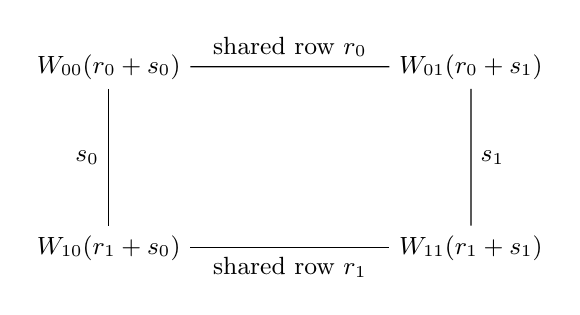
\begin{tikzpicture}[every node/.style={font=\small},scale=1.15]
\node (a) at (0,2) {$W_{00}(r_0+s_0)$};
\node (b) at (4,2) {$W_{01}(r_0+s_1)$};
\node (c) at (0,0) {$W_{10}(r_1+s_0)$};
\node (d) at (4,0) {$W_{11}(r_1+s_1)$};
\draw (a) -- node[above] {shared row $r_0$} (b);
\draw (c) -- node[below] {shared row $r_1$} (d);
\draw (a) -- node[left] {$s_0$} (c);
\draw (b) -- node[right] {$s_1$} (d);
\end{tikzpicture}

\caption{A square after fixing the slice background. The four rows
$r_0,r_1,s_0,s_1$ are independent, but their four sums satisfy one parity
relation. Fourier expansion therefore leaves one common frequency.
Different squares of a collision-free cube use disjoint rows.}
\label{fig:square}
\end{figure}


For four possibly different real slice functions $W_{ab}$, direct
Fourier expansion gives
\begin{equation}\label{eq:square-fourier}
 \E_{r_0,r_1,s_0,s_1}
       \prod_{a,b\in\{0,1\}}W_{ab}(r_a+s_b)
 =\sum_\alpha\prod_{a,b\in\{0,1\}}\widehat W_{ab}(\alpha).
\end{equation}
Indeed averaging $r_0,r_1$ forces the two frequencies in each row
of the square to agree, and averaging $s_0,s_1$ forces agreement
between these rows. Using the coefficient bound on two factors and
Cauchy--Schwarz and Parseval on the other two, the absolute value
of~\eqref{eq:square-fourier} is at most
\begin{equation}\label{eq:square-bound}
 \eps_0^2\sum_\alpha
       |\widehat W_{10}(\alpha)\widehat W_{11}(\alpha)|
 \le\eps_0^2H^2.
\end{equation}

Different squares use disjoint rows in both tables: any change in one
of the other $m-2$ coordinates changes a retained coordinate of
every such row. Conditional on the fixed background, their products
are consequently independent. Their slice functions may share that
background, which does not affect this independence. The absolute
conditional expectation of the full cube product is therefore at most
$(\eps_0^2H^2)^{2^{m-2}}$.
Combining this with the collision bound and
\eqref{eq:box-outer-average}, and using
$(a+b)^{1/Q}\le a^{1/Q}+b^{1/Q}$ for $a,b\ge0$, gives
\begin{equation}\label{eq:pair-correlation}
 \E\mathfrak d_Y(w^{ij})
 \le2A_0(m/\ell)^{1/2^m}
     +\sqrt{H(\gamma+H^2/A_0)}.
\end{equation}
The maximizing face signs were eliminated by the deterministic
inequality before the conditional independence argument was used.
No independence assumption about those signs is involved.

\subsection{Choosing parameters and completing inner decoding}
\label{sec:inner-completion}

For any two fields on a fixed box,
$|\mathfrak d_Y(u)-\mathfrak d_Y(v)|\le\E_{x\in Y}|u_x-v_x|$.
Thus~\eqref{eq:box-restriction}, localization, the processing losses,
and~\eqref{eq:pair-correlation} imply, for each pair class,
\begin{align}
 \E\mathfrak d_X(L^{ij})
 \le{}&\underbrace{\sigma^{-1}
       \sqrt{(s+Rm)\ell/(n-1)}}_{e_{\mathrm{loc}}}
       +\frac{\sigma^{-2}}H
       +\underbrace{\sigma^{-1}\sqrt{C_0/\gamma}
           (\theta^2+mpN/\sigma^2)^{1/4}}_{e_{\mathrm{atom}}}
       \notag\\
      &+\frac{\sigma^{-2}}{A_0}
       +2A_0(m/\ell)^{1/2^m}
       +\sqrt{H(\gamma+H^2/A_0)}.
 \label{eq:six-errors}
\end{align}
For class $0$, the corresponding bound is
\begin{equation}\label{eq:zero-errors}
 \E\mathfrak d_X(L^0)
 \le e_{\mathrm{loc}}+\frac{2\sigma^{-2}}{A_0}
      +2A_0(m/\ell)^{1/2^m}.
\end{equation}

\begin{proof}[Proof of Theorem~\ref{thm:inner}]
The smoothing parameters were fixed in
Proposition~\ref{prop:correlation}. Choose $m$ as in
\eqref{eq:choose-m}, define $d_0$ by~\eqref{eq:class-target}, and set
$e=d_0/10$. Make the following successive choices, each with strict
slack:
\begin{enumerate}[label=\arabic*.,leftmargin=*]
 \item Choose a positive integer $H$ with $\sigma^{-2}/H<e$.
 \item Choose a positive rational $\gamma$ with $H\gamma<e^2/4$.
 \item Choose a positive integer $A_0$ so large that
       $2\sigma^{-2}/A_0<e$ and $H^3/A_0<e^2/4$.
       These choices give
       $\sqrt{H(\gamma+H^2/A_0)}<e$.
 \item Choose an integer $\ell\ge2$ so large that
       $2A_0(m/\ell)^{1/2^m}<e$.
 \item Choose an integer $n>\ell$ so large that
       $\sigma^{-1}\sqrt{(s+Rm)\ell/(n-1)}<e$.
 \item Now $N=n^m$, $M=mn^{m-1}$ and
       $C_0=4^M\binom{N+s}{s}$ are fixed. Choose positive rationals
       $p,\theta<1$ so small that
       \[
        \theta^2+\frac{mpN}{\sigma^2}
        <\frac{e^4\sigma^4\gamma^2}{C_0^2}.
       \]
       This makes $e_{\mathrm{atom}}<e$.
\end{enumerate}
All choices are finite and use explicit inequalities. Roots in these
inequalities can be removed by raising positive quantities to integer
powers, so rational arithmetic and integer search suffice. Neither the
alphabet size nor the distribution of the proof index enters them.

If the row-atom assertion failed for these $p,\theta$, the preceding
argument would apply. Each pair-class correlation in
\eqref{eq:six-errors} would be less than $6e<d_0$, and the class-$0$
correlation in~\eqref{eq:zero-errors} would be less than $3e<d_0$.
Summing over the $1+\binom m2$ classes would give
\[
 \E\mathfrak d_X(L)<(1+\tbinom m2)d_0=\frac1{4T},
\]
contradicting~\eqref{eq:class-correlation-lower}. This proves the
claimed probability at least $p$ of an odd conditional coefficient
of magnitude at least $\theta$. The pointwise bound on $h_x$ is
\eqref{eq:gradient-bounds}, completing
Theorem~\ref{thm:inner}.
\end{proof}
